\chapter{Thermodynamic Properties of Pure Fluids}\label{Chapter:ThermodynamicPropertiesPureFluids}

   \begin{LearningObjectivesBlock}{Learning Objectives}
      Upon completion of this chapter, you will be able to
        \begin{enumerate}
           \item Define pure substances and thermodynamic phases;
           \item State the Gibbs phase rule and its use to define the number of degrees of freedom of a system;
           \item Identify phases and phase transitions in a diagram;
           \item Formulate the solution for thermodynamic problems involving the calculation of volume of pure substances;
           \item Select appropriate equation of state for a given problem/application;
        \end{enumerate}
\medskip
     Recommended reading: Chapters 3 of \citet{SmithVanNess_Book}, 6 of \citet{Sandler_Book}, 2 of \citet{Borgnakke_Book} or 4 of \citet{Atkins_Book}.
   \end{LearningObjectivesBlock}


%%%%%%%%%%%%%%%%%%%%%%%%%%%%%%%%%%%%%%%%%%%%%%%%%%%%%%%%%%%%%%%%%
\begin{comment}
   \begin{LearningObjectivesBlock}{Learning Objectives}
      Upon completion of this chapter, you will be able to
        \begin{enumerate}
           \item {\bf Knowledge:} Define, Name, Select, State 
           \item {\bf Comprehension:} Describe, Identify, Discuss
           \item {\bf Application:} Apply, Demonstrate, Employ, Sketch
           \item {\bf Analysis:} Analyse, Compare, Calculate, Solve
           \item {\bf Synthesis:} Determine, Formulate
           \item {\bf Evaluation:} Assess, Check, Estimate, Compare, Measure, Monitor
        \end{enumerate}
\end{comment}
%%%%%%%%%%%%%%%%%%%%%%%%%%%%%%%%%%%%%%%%%%%%%%%%%%%%%%%%%%%%%%%%%

%%%% ETOC
\localtableofcontents
   

%%% SECTION
\section{Introduction}\label{Chapter:ThermodynamicPropertiesPureFluids:Section:Introduction}
   This chapter is an introduction to some of the mathematical underpinnings of chemical thermodynamics. Practical applications of most of the contents of this chapters may not be promptly obvious, however this is critical to fully understand concepts, theories and practices that will be introduced in later chapters. MORE!!

%%% SECTION
\section{Thermodynamic Property Relations for Single Phase Systems}\label{Chapter:ThermodynamicPropertiesPureFluids:Section:ThermodynamicPropertiesSinglePhase}
     \begin{subequations}

In Chapter~\ref{Chapter:FirstLaw}, we have learnt that the First Law for reversible processes in closed systems can be written as (for $n$ moles),
   \begin{equation}
       d\left(n U\right) = d Q_{\text{rev}} + d W_{\text{rev}},\label{Chapter:ThermodynamicPropertiesPureFluids:Eqn:FirstLaw}
   \end{equation} 
with $d W_{\text{rev}} = -Pd(nV)$ and $d Q_{\text{rev}}=Td(nS)$,
   \begin{equation}
       d\left(n U\right) = T d(nS) - Pd(nV).\label{Chapter:ThermodynamicPropertiesPureFluids:Eqn:FirstSecondLaw}
   \end{equation} 
This relation involves {\it only state functions}, therefore it is not restricted to reversible processes. The only constraint of this relation is that it is defined for closed systems and it assumes that changes may occur between equilibrium states. Finally, Eqn.~\ref{Chapter:ThermodynamicPropertiesPureFluids:Eqn:FirstSecondLaw} involves five thermodynamic properties: $P, T, V, U$ and $S$, and for $n=1$ mol, it becomes,
   \begin{shaded}
     \begin{equation}
        TdS = dU + PdV,\label{Chapter:ThermodynamicPropertiesPureFluids:Eqn:FundamentalRelation01}
     \end{equation}
   \end{shaded}
however, we know the definition of enthalpy,
     \begin{displaymath}
        dH = dU + d(PV) = dU + PdV + VdP.
     \end{displaymath}
Replacing this relation in Eqn.~\ref{Chapter:ThermodynamicPropertiesPureFluids:Eqn:FundamentalRelation01},
   \begin{shaded}
     \begin{equation}
        TdS = dH - VdP.\label{Chapter:ThermodynamicPropertiesPureFluids:Eqn:FundamentalRelation02}
     \end{equation}
   \end{shaded}
Equations~\ref{Chapter:ThermodynamicPropertiesPureFluids:Eqn:FundamentalRelation01}-\ref{Chapter:ThermodynamicPropertiesPureFluids:Eqn:FundamentalRelation02} correlate entropy changes to changes in other thermodynamic properties
      \begin{eqnarray}
         && dU = TdS - PdV \nonumber \\
         && dH = TdS + VdP. \nonumber 
      \end{eqnarray}
These two fundamental relations can be used to define the two remaining thermodynamic potentials, Gibbs ($G$) free and Helmholtz free ($A$) energy functions as:\index{Gibbs free energy! Definition}\index{Helmholtz free energy}
      \begin{eqnarray}
         && A \equiv U -TS \nonumber \\
         && G \equiv H -TS, \nonumber 
      \end{eqnarray}
or in differential form,
      \begin{eqnarray}
        && dA = dU -TdS - SdT \nonumber \\
        && dG = dH -TdS - SdT.\nonumber 
      \end{eqnarray}
Using Eqns.~\ref{Chapter:ThermodynamicPropertiesPureFluids:Eqn:FundamentalRelation01}-\ref{Chapter:ThermodynamicPropertiesPureFluids:Eqn:FundamentalRelation02}:
   \begin{shaded}
      \begin{eqnarray}
        && dA = - SdT - PdV, \label{Chapter:ThermodynamicPropertiesPureFluids:Eqn:HelmholtzFundamentalRelation01}\\ 
        && dG = - SdT + VdP. \label{Chapter:ThermodynamicPropertiesPureFluids:Eqn:GibbsFundamentalRelation01}
      \end{eqnarray}
   \end{shaded}
These four equations, Eqns.~\ref{Chapter:ThermodynamicPropertiesPureFluids:Eqn:FundamentalRelation01}-~\ref{Chapter:ThermodynamicPropertiesPureFluids:Eqn:GibbsFundamentalRelation01} are known as {\it fundamental thermodynamic relations} as they correlate the five thermodynamic potentials -- $U$, $H$, $S$, $G$, and $A$ with $PVT$ properties.\index{Fundamental thermodynamic relations}


     \end{subequations}

%%% SECTION
     \section{Maxwell Relations}\label{Chapter:ThermodynamicPropertiesPureFluids:Section:MaxwellRelations}
     \begin{subequations}

The thermodynamic potentials expressed in the four fundamental relations (Eqns.~\ref{Chapter:ThermodynamicPropertiesPureFluids:Eqn:FundamentalRelation01}-~\ref{Chapter:ThermodynamicPropertiesPureFluids:Eqn:GibbsFundamentalRelation01}) can be defined as a general functional, 
   \begin{displaymath}
    f = f(a,b),
   \end{displaymath}
with the assumption that the thermodynamic potentials, $f$, are continuous (and differentiable) throughout the domain. Therefore, we can write the total derivative\footnote{Total derivative along with the main elements of Calculus is briefly defined in Appendix~\ref{Appendix_Calculus:TotalDifferential}.} of function $f$ as
   \begin{equation}
         df = \underbrace{\left(\frc{\partial f}{\partial a}\right)_{b}}_{M}da + \underbrace{\left(\frc{\partial f}{\partial b}\right)_{a}}_{N}db = Mda + Ndb.\label{Chapter:ThermodynamicPropertiesPureFluids:Eqn:EqualRelation0}
   \end{equation}
Now, if we differentiate $M$ \wrt $b$ and $N$ \wrt $a$,
   \begin{displaymath}
         \left(\frc{\partial M}{\partial b}\right)_{a} = \frc{\partial^{2}f}{\partial a\partial b} \;\;\;\text{ and }\;\;\; \left(\frc{\partial N}{\partial a}\right)_{b} = \frc{\partial^{2}f}{\partial b\partial a},
   \end{displaymath}
since we required that $f(a,b)$ to be \underline{continuous}, 
   \begin{equation}
         \frc{\partial^{2}f}{\partial a\partial b} = \frc{\partial^{2}f}{\partial b\partial a}\;\;\Longrightarrow \left(\frc{\partial M}{\partial b}\right)_{a} = \left(\frc{\partial N}{\partial a}\right)_{b}\label{Chapter:ThermodynamicPropertiesPureFluids:Eqn:EqualRelation}
   \end{equation}
Now applying Eqn.~\ref{Chapter:ThermodynamicPropertiesPureFluids:Eqn:EqualRelation} into ~\ref{Chapter:ThermodynamicPropertiesPureFluids:Eqn:FundamentalRelation01},
   \begin{displaymath}
       \begin{cases}
          df = Mda + Ndb, & \\
          dU = TdS - PdV, &
       \end{cases}
   \end{displaymath}
with $M=T$, $da=dS$, $N=-P$, $db = dV$ and $df = dU$ leading to,
      \begin{shaded}
         \begin{equation}
            \left(\frc{\partial M}{\partial b}\right)_{a} = \left(\frc{\partial N}{\partial a}\right)_{b} \;\;\;\Longrightarrow \left(\frc{\partial T}{\partial V}\right)_{S} = - \left(\frc{\partial P}{\partial S}\right)_{V}\label{Chapter:ThermodynamicPropertiesPureFluids:Eqn:MaxwellRelation1}
         \end{equation}
Using the same procedure with  Eqn.~\ref{Chapter:ThermodynamicPropertiesPureFluids:Eqn:FundamentalRelation02}-~\ref{Chapter:ThermodynamicPropertiesPureFluids:Eqn:GibbsFundamentalRelation01},
           \begin{eqnarray}
              \left(\frc{\partial T}{\partial P}\right)_{S} &=& \left(\frc{\partial V}{\partial S}\right)_{P},\label{Chapter:ThermodynamicPropertiesPureFluids:Eqn:MaxwellRelation2} \\
              \left(\frc{\partial S}{\partial V}\right)_{T} &=& \left(\frc{\partial P}{\partial T}\right)_{V},\label{Chapter:ThermodynamicPropertiesPureFluids:Eqn:MaxwellRelation3} \\
              -\left(\frc{\partial S}{\partial P}\right)_{T} &=& \left(\frc{\partial V}{\partial T}\right)_{P},\label{Chapter:ThermodynamicPropertiesPureFluids:Eqn:MaxwellRelation4} 
           \end{eqnarray}
      \end{shaded}
Equations~\ref{Chapter:ThermodynamicPropertiesPureFluids:Eqn:MaxwellRelation1}-~\ref{Chapter:ThermodynamicPropertiesPureFluids:Eqn:MaxwellRelation4} are called as \blue{Maxwell relations}, and they allow determining changes in entropy without directly measurement, but only with changes on the PVT properties. We can also make use of the total derivative definition and apply it into Eqns.~\ref{Chapter:ThermodynamicPropertiesPureFluids:Eqn:FundamentalRelation01}-~\ref{Chapter:ThermodynamicPropertiesPureFluids:Eqn:GibbsFundamentalRelation01}, thus
   \begin{eqnarray}
                      &                            df =  \left(\frc{\partial f}{\partial a}\right)_{b}da + \left(\frc{\partial f}{\partial b}\right)_{a}db& \nonumber \\
      dU = TdS - PdV  &\;\;\;\Longleftrightarrow \;\;\;& dU =  \underbrace{\left(\frc{\partial U}{\partial S}\right)_{V}}_{T}dS + \underbrace{\left(\frc{\partial U}{\partial V}\right)_{S}}_{-P}dV \nonumber \\
      dH = TdS + VdP  &\;\;\;\Longleftrightarrow \;\;\;& dH =  \underbrace{\left(\frc{\partial H}{\partial S}\right)_{P}}_{T}dS + \underbrace{\left(\frc{\partial H}{\partial P}\right)_{S}}_{V}dP \nonumber \\
      dA = -SdT - PdV &\;\;\;\Longleftrightarrow \;\;\;& dA =  \underbrace{\left(\frc{\partial A}{\partial T}\right)_{V}}_{-S}dT + \underbrace{\left(\frc{\partial A}{\partial V}\right)_{T}}_{-P}dV \nonumber \\
      dG = -SdT + VdP &\;\;\;\Longleftrightarrow \;\;\;& dG =  \underbrace{\left(\frc{\partial G}{\partial T}\right)_{P}}_{-S}dT + \underbrace{\left(\frc{\partial G}{\partial P}\right)_{T}}_{V}dP \nonumber 
   \end{eqnarray}
Therefore
   \begin{shaded}
         \begin{eqnarray}
             \left(\frc{\partial U}{\partial S}\right)_{V} & =  T = & \left(\frc{\partial H}{\partial S}\right)_{P}\label{Chapter:ThermodynamicPropertiesPureFluids:Eqn:MaxwellRelation5} \\
             \left(\frc{\partial U}{\partial V}\right)_{S} & = -P = & \left(\frc{\partial A}{\partial V}\right)_{T}\label{Chapter:ThermodynamicPropertiesPureFluids:Eqn:MaxwellRelation6} \\
             \left(\frc{\partial H}{\partial P}\right)_{S} & =  V = & \left(\frc{\partial G}{\partial P}\right)_{T}\label{Chapter:ThermodynamicPropertiesPureFluids:Eqn:MaxwellRelation7} \\
             \left(\frc{\partial A}{\partial T}\right)_{V} & = -S = & \left(\frc{\partial G}{\partial T}\right)_{P}\label{Chapter:ThermodynamicPropertiesPureFluids:Eqn:MaxwellRelation8}
         \end{eqnarray}
   \end{shaded}
These property relations, Eqns.~\ref{Chapter:ThermodynamicPropertiesPureFluids:Eqn:MaxwellRelation5}-~\ref{Chapter:ThermodynamicPropertiesPureFluids:Eqn:MaxwellRelation8}, easily correlate measurable properties ($P$, $V$ and $T$) with non-measurable potentials ($U$, $H$, $S$, $A$ and $G$).

      \end{subequations}


   % Example
   \begin{MyExample}{\begin{center}{\bf Example}\end{center}}
     \begin{example}\label{Chapter:ThermodynamicPropertiesPureFluids:Example1} \citep{Balmer_Book}
         Suppose we make a series of measurements in the laboratory and think we discovered a new thermodynamic property, call it $\eta$. Our experimental data provide an empirical equation of the form,
          \begin{displaymath}
             d\eta = PdV + V^{2}dP
          \end{displaymath}
          Is $\eta$ a new property?
     \end{example}

% SOLUTION
       \noindent{\bf Solution:}
        The unknown is whether or not $\eta$ is a new thermodynamic property. Using Eqn.~\ref{Chapter:ThermodynamicPropertiesPureFluids:Eqn:EqualRelation0},
        \begin{displaymath}
            d\eta = Mda + Ndb = PdV + V^{2}dP,
        \end{displaymath}
        with $M=P$, $N=V^{2}$, $a=V$ and $b=P$. The cross differentials are
        \begin{displaymath}
            \Partial[M]{b}{a} = \Partial[P]{P}{V} = 1\;\;\;\text{ and }\;\;\; \Partial[N]{a}{b} = \Partial[V^{2}]{V}{P} = 2V \ne \Partial[M]{b}{a}.
        \end{displaymath}
         Since this equality is not satisfied, $\eta$ can not be a thermodynamic property.
   \end{MyExample}
   
   % Example
   \begin{MyExample}{\begin{center}{\bf Example}\end{center}}
     \begin{example}\label{Chapter:ThermodynamicPropertiesPureFluids:Example2} 
         A block of copper of 1 kg undertakes a reversible compression from 0.1 MPa to 100 MPa at constant temperature of 15$^{\circ}$C. Calculate:
    \begin{enumerate}[a)]
       \item Work done on the copper block during the process;
       \item Change in entropy {\it per} kg of copper;
       \item Heat transfer and;
       \item Change of internal energy {\it per} kg.
    \end{enumerate}
    Given, 
    \begin{itemize}
       \item Volume expansivity coefficient: $\beta = 5\times 10^{-5}$ K$^{-1}$;
       \item Isothermal compressibility coefficient: $\kappa = 8.6\times 10^{-12}$ m$^{2}$.N$^{-1}$;
       \item specific volume: $v=1.14\times 10^{-4}$ m$^{3}$.kg$^{-1}$.
    \end{itemize} 
     \end{example}

% SOLUTION
       \noindent{\bf Solution:}
       \begin{enumerate}[a)]
%
            \item The work done during the compression,
                \begin{displaymath}
                   w = -\int P dv,
                \end{displaymath}
                where $v$ is the specific volume. $\kappa$ was defined in Eqn.~\ref{Chapter:VolumetricPropertiesPureSubstances:Eqn:CompressibilityExpansivity} as,
                \begin{displaymath}
                   \kappa = \frc{1}{v}\left(\frc{\partial v}{\partial P}\right)_{T}\;\Longrightarrow \; v\kappa dP = - dv \;\;\text{ (with constant T)}
                \end{displaymath}
                For isothermal processes
                \begin{displaymath}
                   w = -\int P dv = - \int P\left(-v\kappa dP\right) = \frc{v}{2}\kappa\left(P_{2}^{2}-P_{1}^{2}\right) = 4.90\text{ J.kg}^{-1}
                \end{displaymath}
%
            \item $ds$ = ? (specific entropy).\\
                  From the Maxwell relations -- Eqn.~\ref{Chapter:ThermodynamicPropertiesPureFluids:Eqn:MaxwellRelation4}, 
                \begin{displaymath}
                   -\left(\frc{\partial s}{\partial P}\right)_{T} = \left(\frc{\partial v}{\partial T}\right)_{P},
                \end{displaymath}
                and from the definition of $\beta$,
                \begin{eqnarray}
                    && \beta = \frc{1}{v}\left(\frc{\partial v}{\partial T}\right)_{P} \;\;\Longrightarrow\;\; -\left(\frc{\partial s}{\partial P}\right)_{T} = \beta v \nonumber \\
                    && ds = -\beta v dP \;\;\Longrightarrow ds = s_{2}-s_{1} = -\beta v \left(P_{2}-P_{1}\right) = -0.5694 \text{ J.(kg.K)}^{-1} \nonumber
                \end{eqnarray}
%
            \item The heat transferred in such reversible isothermal process is
                \begin{displaymath}
                   dq = Tds \;\;\Longrightarrow q = T\left(s_{2}-s_{1}\right) = -164.07 \text{ J.kg}^{-1}.
                \end{displaymath}
%
            \item The specific internal energy,
                \begin{eqnarray}
                   &&  du = q + w \nonumber \\
                   && \left(u_{2}-u_{1}\right) = \underbrace{-164.07}_{\text{heat removed from the system}} + \overbrace{4.90}^{\text{work given to the system}} = -159.17 \text{ J.kg}^{-1}. \nonumber
                \end{eqnarray}
       \end{enumerate}
   \end{MyExample}
   

   % Example
   \begin{MyExample}{\begin{center}{\bf Example}\end{center}}
     \begin{example}\label{Chapter:ThermodynamicPropertiesPureFluids:Example3}  
     Demonstrate that the derivative of molar volume \wrt temperature at constant pressure is
     \begin{displaymath}
         \Partial[V]{T}{P} = -\frc{\Partial[P]{T}{V}}{\Partial[P]{V}{T}},
     \end{displaymath}
     and obtain an expression, $\Partial[V]{T}{P}$, for the van der Waals EOS. 

     \noindent{\bf Hint:} You should start the proof from the total differential of a continuous function $f(a,b)$,
     \begin{displaymath}
         df = \Partial[f]{a}{b}da + \Partial[f]{b}{a}db.
     \end{displaymath}
     \end{example}

% SOLUTION
       \noindent{\bf Solution:}
     The total differential of a generic continuous function $f(a,b)$ is
     \begin{displaymath}
         df = \Partial[f]{a}{b}da + \Partial[f]{b}{a}db.
     \end{displaymath}
     where (from the given thermodynamic function) $f=P$, $a=T$ and $b=V$, \ie
     \begin{displaymath}
         dP = \Partial[P]{T}{V}dT + \Partial[P]{V}{T}dV.
     \end{displaymath}
     However we want a differential expression in which $P$ is constant, therefore $dP = 0$,
     \begin{eqnarray}
         0 &=& \Partial[P]{T}{V}dT + \Partial[P]{V}{T}dV \;\;\;\text{ at } P \text{ constant},\nonumber \\
         \Partial[V]{T}{P} &=& -\frc{\Partial[P]{T}{V}}{\Partial[P]{V}{T}}.\nonumber
     \end{eqnarray}

     \medskip\noindent
     The vdW-EOS is,
     \begin{displaymath}
          P = \frc{RT}{V-b} - \frc{a}{V^{2}},
     \end{displaymath}
     where $V$ is the molar volume and $a$ and $b$ are constants that {\it depends only on critical properties}, $P_{c}$ and $T_{c}$. Due to the non-linearity of this EOS, obtaining $\Partial[V]{T}{P}$ from a direct differentiation would be difficult. However, we can use the expression that we just derived,
     \begin{displaymath}
         \Partial[V]{T}{P} = -\frc{\Partial[P]{T}{V}}{\Partial[P]{V}{T}} = -\frc{\frc{R}{V-b}}{-\frc{RT}{\left(V-b\right)^{2}}+\frc{2a}{V^{3}}}
     \end{displaymath} 

   \end{MyExample}


%%% SECTION
   \section{Relations for Internal Energy, Enthalpy and Entropy}\label{Chapter:ThermodynamicPropertiesPureFluids:Section:U_H_S_Relations}
      \begin{subequations}

Maxwell relations can help to develop relations for changes in $U$, $H$ and $S$ that reflect in heat and work interactions. Given
    \begin{displaymath}
       \begin{cases}
           H = H(T,P), & \text{ and } \\
           S = S(T,P), &
        \end{cases} 
    \end{displaymath}
    \ie defining {\it enthalpy} and {\it entropy} as functions of temperature and pressure. Using Eqn.~\ref{Chapter:ThermodynamicPropertiesPureFluids:Eqn:FundamentalRelation02},
    \begin{displaymath}
      dH = TdS + VdP,
    \end{displaymath}
    at constant pressure and multiplying by $(1/dT)$,
    \begin{eqnarray}
        \Partial[H]{T}{P} &=& C_{p} = T\Partial[S]{T}{P} \nonumber \\
        \Partial[S]{T}{P} &=& \frc{C_{p}}{T}.\label{Chapter:ThermodynamicPropertiesPureFluids:Section:DerivedEntropyRelation1}
    \end{eqnarray}
Nowm using Eqn.~\ref{Chapter:ThermodynamicPropertiesPureFluids:Eqn:FundamentalRelation02} at constant $T$, multiplied by $(1/dP)$,
    \begin{displaymath}
       \Partial[H]{P}{T} = T\underbrace{\Partial[S]{P}{T}}_{\text{Eqn.~\ref{Chapter:ThermodynamicPropertiesPureFluids:Eqn:MaxwellRelation4}}} + V = -T\Partial[V]{T}{P} + V.
    \end{displaymath}
    
      \begin{shaded}
Now if we write the total derivative of function $H$,
    \begin{displaymath}
       dH = \Partial[H]{T}{P}dT + \Partial[H]{P}{T}dP 
    \end{displaymath}
         \begin{equation}
            dH = C_{p}dT + \left[V - T\Partial[V]{T}{P}\right]dP.\label{Mod03_DerivedEnthalpyRelation1}
         \end{equation}
      \noindent
And the total derivative of function $S$ can be expressed as (using Eqn.~\ref{Chapter:ThermodynamicPropertiesPureFluids:Section:DerivedEntropyRelation1}),
      \begin{displaymath}
         dS = \underbrace{\Partial[S]{T}{P}}_{\text{Eqn.~\ref{Chapter:ThermodynamicPropertiesPureFluids:Section:DerivedEntropyRelation1}}}dT + \overbrace{\Partial[S]{P}{T}}^{\text{Eqn.~\ref{Chapter:ThermodynamicPropertiesPureFluids:Eqn:MaxwellRelation4}}}dP 
       \end{displaymath}
          \begin{equation}
             dS = C_{p}\frc{dT}{T} - \Partial[V]{T}{P}dP\label{Mod03_DerivedEntropyRelations}
          \end{equation}
       \end{shaded}

\medskip

\begin{shaded}
      \noindent
      For an \blue{ideal gas}, $V=\frac{RT}{P}$ and $\Partial[V]{T}{P} = \frc{R}{P}$, therefore Eqn.~\ref{Mod03_DerivedEnthalpyRelation1} becomes
         \begin{eqnarray}
            dH &=& C_{p}dT + \left[V-\overbrace{T\frc{R}{P}}^{=V}\right]dP \nonumber \\
            dH &=& C_{p}dT,\label{Mod03_DerivedEnthalpyRelation2}
         \end{eqnarray}
      and Eqn.~\ref{Mod03_DerivedEntropyRelations} becomes,
         \begin{equation}
            dS = C_{p}\frc{dT}{T} -\frc{R}{P}dP.\label{Mod03_DerivedEntropyRelations2}
         \end{equation}
\end{shaded}

\bigskip

Similarly, we can express $U$ and $S$ as functions of $T$ and $V$,
    \begin{displaymath}
       \begin{cases}
           U = U(T,V), & \text{ and } \\
           S = S(T,V), &
        \end{cases}
    \end{displaymath} 
using the same procedure as above starting from the derivatives of functions $U$ and $S$,
    \begin{eqnarray}
        dU &=& \Partial[U]{T}{V}dT + \Partial[U]{V}{T}dV, \text{ and } \nonumber \\
        dS &=& \Partial[S]{T}{V}dT + \Partial[S]{V}{T}dV. \nonumber
    \end{eqnarray} 
From Eqn.~\ref{Chapter:ThermodynamicPropertiesPureFluids:Eqn:FundamentalRelation01}, 
    \begin{displaymath}
        dU = TdS - PdV,
        \begin{cases}
            \red{\times\Partial[]{T}{V}} \Longrightarrow \Partial[U]{T}{V} = T\Partial[S]{T}{V} = C_{v} \Longrightarrow  \Partial[S]{T}{V} = \frc{C_{v}}{T}\\
            \red{\times\Partial[]{V}{T}} \Longrightarrow \underbrace{\Partial[U]{V}{T}}_{\text{Eqn.~\ref{Chapter:ThermodynamicPropertiesPureFluids:Eqn:MaxwellRelation3}}} = T\Partial[S]{V}{T} - P \Longrightarrow \Partial[U]{V}{T} = T\Partial[P]{T}{V}-P   \\
        \end{cases}
    \end{displaymath}
Substituting these relations in the total differentials,
\begin{shaded}
  
          \begin{eqnarray}
             dU = \Partial[U]{T}{V}dT + \Partial[U]{V}{T}dV \;\;&\Longrightarrow&\;\; dU = C_{v}dT + \left[T\Partial[P]{T}{V}-P\right]dV\label{Mod03_DerivedIntEnergyRelation1} \\
             dS = \Partial[S]{T}{V}dT + \Partial[S]{V}{T}dV \;\;&\Longrightarrow&\;\; dS = \frc{C_{v}}{T}dT + \Partial[P]{T}{V}dV.\label{Mod03_DerivedEntropyRelations3}
          \end{eqnarray} 
    \end{shaded}

Equation~\ref{Mod02_Compressibilityexpansivity2} (Module~\ref{Section:02}) relates the isothermal compressibility, $\kappa$, expansivity, $\beta$ coefficients to $T$, $P$ and $V$,
     \begin{eqnarray}
        \frc{dV}{V} &=& \beta dT - \kappa dP \;\;\;\red{\times\Partial[]{T}{V} \nonumber \text{ \ie at }V\text{ constant}} \nonumber \\
            0       &=& \beta - \kappa\Partial[P]{T}{V} \Longrightarrow \Partial[P]{T}{V} = \frc{\beta}{\kappa} \nonumber
     \end{eqnarray}
This relation can be used in Eqns.~\ref{Mod03_DerivedIntEnergyRelation1} and~\ref{Mod03_DerivedEntropyRelations3},
     \begin{eqnarray}
        dU &=& C_{v}dT + \left[T\frc{\beta}{\kappa}-P\right]dV\label{Mod03_DerivedIntEnergyRelation2} \\
        dS &=& \frc{C_{v}}{T}dT + \frc{\beta}{\kappa}dV.\label{Mod03_DerivedEntropyRelations4}
     \end{eqnarray}

\begin{table}[h]
   \begin{shaded} 
       \begin{center}
           {\bf $\kappa$ and $\beta$ Relations for Liquids}
       \end{center}
       \begin{subequations}
          For liquids, using $\beta$ and $\kappa$ in Eqns.~\ref{Mod03_DerivedEnthalpyRelation1}-~\ref{Mod03_DerivedEntropyRelations},
            \begin{eqnarray}
               \Partial[S]{P}{T} &=& -\Partial[V]{T}{P} = -\beta V \nonumber \\
               \Partial[H]{P}{T} &=& V - T\Partial[V]{T}{P} = V - TV\beta = \left(1-\beta T\right)V, \nonumber
            \end{eqnarray}
          leading to
            \begin{eqnarray}
               dH &=& C_{p}dT + \left(1-\beta T\right)VdP \label{Mod03_DerivedEnthalpyLiquid}\\
               dS &=& C_{p}\frc{dT}{T} - \beta V dP.\label{Mod03_DerivedEntropyRelationsLiquid}
            \end{eqnarray}
          For internal energy, we can write,
            \begin{eqnarray}
               dU &=& dH - d(PV) = dH -PdV -VdP\;\;\;\;\blue{\times\Partial[]{P}{T}} \nonumber \\
               \Partial[U]{P}{T} &=& \underbrace{\Partial[H]{P}{T}}_{\red{\cancel{V}}-T\Partial[V]{T}{P}} - P\Partial[V]{P}{T} - \red{\cancel{V}} \nonumber \\
                                 &=& - T\underbrace{\Partial[V]{T}{P}}_{\beta V} - P \underbrace{\Partial[V]{P}{T}}_{\kappa V} \nonumber \\
               \Partial[U]{P}{T} &=& \left(\kappa P - \beta T\right)V \label{Mod03_DerivedInternalEnergyLiquid}
            \end{eqnarray}
          \underline{These relations are only applied to {\it liquids}.}
       \end{subequations}
    \end{shaded}
\end{table}
      \end{subequations}

%%% SECTION
\section{Gibbs Free Energy as Generating Function}\label{Section:03:GibbsGeneratingFunction}

The fundamental relation for the Gibbs free energy, Eqn.~\ref{Chapter:ThermodynamicPropertiesPureFluids:Eqn:GibbsFundamentalRelation01}, demonstrated that this potential can be expressed as a function of temperature and pressure, $G=G(T,P)$. In chemical industrial (or lab) processes, both properties, $T$ and $P$, can be readily measured and controlled, and therefore used to obtain $G$. A convenient way to deal with this relation is rewriting it in dimensionless form
    \begin{eqnarray}
         d\left(\frc{G}{RT}\right) &\equiv& \frc{1}{RT}dG - \frc{GR}{\left(RT\right)^{2}}dT = \frc{1}{RT}\underbrace{dG}_{\text{using Eqn.~\ref{Chapter:ThermodynamicPropertiesPureFluids:Eqn:GibbsFundamentalRelation01}}} - \overbrace{\frc{G}{RT^{2}}}^{\text{using }G=H-TS}dT \nonumber \\
                                    & =& \frc{V}{RT}dP - \red{\cancel{\frc{S}{RT}dT}} - \frc{H}{RT^{2}}dT + \red{\cancel{\frc{S}{RT}dT}} \nonumber
    \end{eqnarray}

    \begin{subequations}
       \begin{shaded} 
          \begin{eqnarray}
              && d\left(\frc{G}{RT}\right) = \frc{V}{RT}dP - \frc{H}{RT^{2}}dT\label{Mod03_GibbsGeneratingFunction} \\
              && \frc{V}{RT} = \Partial[(G/RT)]{P}{T} \;\;\blue{\text{ for } T\text{ constant}},\label{Mod03_GibbsGeneratingFunctionTConst} \\
              && \frc{H}{RT} = -T\Partial[(G/RT)]{T}{P} \;\;\blue{\text{ for } P\text{ constant}}.\label{Mod03_GibbsGeneratingFunctionPConst}
          \end{eqnarray}
        \end{shaded}
        With a similar procedure we can obtain generating functions from
        \begin{shaded}
           \begin{eqnarray}
              \frc{S}{R} &=& \frc{H}{RT} - \frc{G}{RT}   \;\;\blue{\Longleftarrow \; G=H-TS \;\;\times(1/RT)}\label{Mod03_EntropyGeneratingFunction} \\
              \frc{U}{RT} &=& \frc{H}{RT} - \frc{PV}{RT} \;\;\blue{\Longleftarrow \; U=H-PV \;\;\times(1/RT)}\label{Mod03_IntEnergyGeneratingFunction}
           \end{eqnarray}
        \end{shaded}
    \end{subequations}


%%% SECTION
\section{Residual Properties}\label{Section:03:ResidualProperties}

Another way to calculate energy and entropy changes for real gases is by defining {\it residual properties}, \ie the difference between any extensive thermodynamic property, $M$ (\eg $V$, $U$, $H$, $S$, $G$ and $A$), in real gases and its equivalent assuming ideal gas behaviour, $M^{\text{ig}}$,
   \begin{shaded}
      \begin{displaymath}
         M^{R} \equiv M - M^{\text{ig}},
      \end{displaymath}
   \end{shaded}
thus \eg
   \begin{subequations}
      \begin{equation}
         V^{R} = V - V^{\text{ig}} = \underbrace{V}_{=\frac{zRT}{P}} - \frc{RT}{P} = \frc{RT}{P}\left(Z-1\right).\label{Mod03_ResidualProperties_V}
      \end{equation}
      The {\it residual properties} concept is \underline{only} used for gases, and it is based in the idea that properties of real gases are often close of ideal gas behaviour at similar conditions. We can use the {\it generating function} concept, defined in Section~\ref{Section:03:GibbsGeneratingFunction}, to compute changes in properties based on the Gibbs free energy (Eqn.~\ref{Mod03_GibbsGeneratingFunction}),
      \begin{shaded}
         \begin{equation}
            d\left(G^{R}/RT\right) = d\left(G/RT\right) - d\left(G^{\text{ig}}/RT\right) = \frc{V^{R}}{RT}dP - \frc{H^{R}}{RT^{2}}dT\label{Mod03_ResidualProperties_GeneratingGibbsFunction1}
         \end{equation}
      \end{shaded}
    \end{subequations}

%%% SUBSECTION
   \subsection{Properties obtained at Constant Temperature}

      For processes at constant temperature, \ie, $dT=0$,
          \begin{displaymath}
              d\left(G^{R}/RT\right) = \frc{V^{R}}{RT}dP,
          \end{displaymath}
          integrating from $0$ (ideal gas state) to $P$,
          \begin{eqnarray}
              \left(\frc{G^{R}}{RT}\right)_{P} &-&  \underbrace{\left(\frc{G^{R}}{RT}\right)_{P=0}}_{\Phi \text{ (integration constant)}} =  \int\limits_{0}^{P}\overbrace{\frc{V^{R}}{RT}}^{\text{replacing by Eqn.~\ref{Mod03_ResidualProperties_V}}}dP, \nonumber \\
              \left(\frc{G^{R}}{RT}\right)_{P} &=& \Phi + \int\limits_{0}^{P}\left(Z-1\right)\frc{dP}{P},\label{Mod03_ResidualProperties_GeneratingGibbsFunction2}
          \end{eqnarray}
          Differentiating this expression \wrt $T$ $\left(\text{\ie }\Partial[]{T}{}\right)$ 
          \begin{displaymath}
              \Partial[\left(G^{R}/RT\right)]{T}{} = \int\limits_{0}^{P} \left.\Partial[Z]{T}{}\right|_{P}\frc{dP}{P},
          \end{displaymath}
          here it is important to note that in $\left.\Partial[Z]{T}{}\right|_{P}$, the index $P$ indicates that the differential in brackets is only valid for $P\ne0$, as for $P=0$ the gas is assumed ideal and $Z$ is constant equal to $1$. Now using Eqn.~\ref{Mod03_GibbsGeneratingFunctionPConst},
          \begin{subequations}
          \begin{shaded}
             \begin{equation}
                \frc{H^{R}}{RT} = - T\int\limits_{0}^{P}\left.\Partial[Z]{T}{}\right|_{P}\frc{dP}{P}.\label{Mod03_ResidualProperties_GeneratingEnthalpyFunction2}
             \end{equation}
          \end{shaded}
          With this expression, one can readily obtain the residual enthalpy of a real gas assuming that $\frac{\partial Z}{\partial T}$ at a prescribed pressure can be obtained by experiments or by differentiating the cubic form in $Z$ of any EOS (Eqns.~\ref{Mod02_GeneralEOS}-~\ref{Mod02_Zvap}). Now, using the fundamental relation $G = H - TS$,
          \begin{eqnarray}
                 G^{\text{ig}} &=& H^{\text{ig}} - TS^{\text{ig}} \nonumber \\
                 G^{R} &=& H^{R} - TS^{R}\;\;\;\;\;\blue{\times\frc{1}{RT}} \;\;\;\Longrightarrow \;\;\; \frc{S^{R}}{R} = \frc{H^{R}}{RT} - \frc{G^{R}}{RT} \nonumber \\
                 \frc{S^{R}}{R} &=& \underbrace{-T\int\limits_{0}^{P}\left.\Partial[Z]{T}{}\right|_{P}\frc{dP}{P}}_{\text{Eqn.~\ref{Mod03_ResidualProperties_GeneratingEnthalpyFunction2}}} \overbrace{- \Phi - \int\limits_{0}^{P}\left(Z-1\right)\frc{dP}{P}}^{\text{Eqn.~\ref{Mod03_ResidualProperties_GeneratingGibbsFunction2}}}\;\;\;\blue{(\text{at constant}\;\; T)}.\nonumber %\label{Mod03_ResidualProperties_GeneratingEntropyFunction1}
          \end{eqnarray}
          For practical applications we often require $\Delta S$,
          \begin{displaymath}
             \Delta S = S_{2} - S_{1} = \left(S_{2}^{\text{ig}}-S_{1}^{\text{ig}}\right) + \underbrace{\overbrace{\left(S_{2}^{R}-S_{1}^{R}\right)}^{\Phi\text{ cancels out !!}}}_{\text{Thus we can arbitrarily set }\Phi=0}
          \end{displaymath}
          Thus
          \begin{shaded}
              \begin{eqnarray}
                  \frc{S^{R}}{R} &=& -T\int\limits_{0}^{P}\left.\Partial[Z]{T}{}\right|_{P}\frc{dP}{P} - \int\limits_{0}^{P}\left(Z-1\right)\frc{dP}{P},\label{Mod03_ResidualProperties_GeneratingEntropyFunction2} \\
                  \frc{G^{R}}{RT} &=&  \int\limits_{0}^{P}\left(Z-1\right)\frc{dP}{P}.\label{Mod03_ResidualProperties_GeneratingGibbsFunction3} 
              \end{eqnarray}
          \end{shaded}
       \end{subequations}
          
%%% SUBSECTION
   \subsection{Residual Properties in the Zero-Pressure Limit}
      
       By definition, at pressures near to zero, \ie $P\rightarrow 0$, the gas behaves as an ideal gas and $Z\rightarrow 1$. However, \underline{not all} residual properties become zero near the near-zero pressure condition. Molar volume for example,
       \begin{displaymath}
           \lim\limits_{P\rightarrow 0}V^{R} = \lim\limits_{P\rightarrow 0}V - \lim\limits_{P\rightarrow 0}V^{\text{ig}},
       \end{displaymath}
both terms in the r.h.s. tends to $+\infty$ and the difference is assumed undetermined. For other properties:
       \begin{displaymath}
          \begin{cases}
             \lim\limits_{P\rightarrow 0}H^{R} = 0, & \forall T \text{ (for all $T$)}, \\
             \lim\limits_{P\rightarrow 0}\left(G^{R}/RT\right) = \infty-\infty,& \text{undetermined but not necessarily zero}.  
          \end{cases}
       \end{displaymath}


%%% SUBSECTION
\section{Two-Phase Systems}\label{Section:03:Two_Phase}

%%% SUBSECTION
   \subsection{Clapeyron Relations}\label{Section:03:ClapeyronRelations}

\begin{subequations}
When a pure component is in phase equilibrium, {\it all coexisting phases have the same temperature and pressure}. Therefore, the following criterion is applied,
      \begin{displaymath}
          dG = VdP - SdT = 0 \;\;\;\;\text{ at constant } T \text{ and } P.
      \end{displaymath}
This means that changes in Gibbs free energy in all coexisting phases are the same, \ie,
      \begin{displaymath}
          dG^{\alpha} = dG^{\beta} = dG^{\gamma} = \cdots,
      \end{displaymath}
where $\alpha$, $\beta$, $\gamma$, $\cdots$, are phases in thermodynamic equilibrium. Therefore we can write Gibbs change for two given phases as,
      \begin{displaymath}
          V^{\alpha}dP^{\text{sat}} - S^{\alpha}dT = V^{\beta}dP^{\text{sat}} - S^{\beta}dT.
      \end{displaymath}
$P^{\text{sat}}$ is the saturated pressure, \ie pressure in which phase change occurs. We can manipulate this expression,
      \begin{displaymath}
          \frc{dP^{\text{sat}}}{dT} = \frc{S^{\beta}-S^{\alpha}}{V^{\beta}-V^{\alpha}} = \frc{\Delta S^{\alpha\beta}}{\Delta V^{\alpha\beta}}.
      \end{displaymath}
We can define the {\it latent heat of phase transition} (\eg vaporisation, solidification etc), $\Delta H^{\alpha\beta}$ from Eqn.~\ref{Chapter:ThermodynamicPropertiesPureFluids:Eqn:FundamentalRelation02} integrating with constant pressure,
      \begin{displaymath}
          dH = TdS + VdP \;\;\Rightarrow \;\; \int\limits_{H^{\alpha}}^{H^{\beta}} dH = \int\limits_{S^{\alpha}}^{S^{\beta}} TdS \;\;\Rightarrow \;\;  H^{\beta}-H^{\alpha} = T\left(S^{\beta}-S^{\alpha}\right)  \;\;\Rightarrow \;\; \Delta H^{\alpha\beta} = T\Delta S^{\alpha\beta},
      \end{displaymath}
therefore,
      \begin{shaded}
          \begin{equation}
              \frc{dP^{\text{sat}}}{dT} = \frc{\Delta H^{\alpha\beta}}{T\Delta V^{\alpha\beta}},\label{Mod03_ClapeyronEqn} 
          \end{equation}
          this expression is known as {\it Clapeyron Equation} and it expresses the relation between a change in temperature and a change in pressure under the conditions of equilibrium between two phases. 
      \end{shaded}

We can determine the enthalpy of vaporisation (\ie latent heat of vaporisation), $H^{\alpha\beta}=H^{\text{fg}}$, at a given $T$ by simply measuring the slope of the saturation curve on a $PT$ diagram (Fig.~\ref{Mod03Fig01}) and the specific volume of saturated liquid and saturated vapour at the given $T$. The {\it Clapeyron Equation} can be simplified for liquid-vapour (and for solid-vapour) phase changes, at low pressures
      \begin{displaymath}
         V^{\text{g}} >>>> V^{\text{f}} \;\;\Longrightarrow \;\; V^{\text{fg}} = V^{\text{g}},
      \end{displaymath}
if we treat the vapour as an ideal gas, $V^{\text{g}} = \frc{RT}{P}$, and replacing in Eqn.~\ref{Mod03_ClapeyronEqn} 
      \begin{displaymath}
          \frc{dP^{\text{sat}}}{dT} = \frc{P^{\text{sat}}\Delta H^{\text{fg}}}{RT^{2}} \;\;\;\Longrightarrow \;\;\; \left(\frc{dP}{P}\right)_{\text{sat}} = \frc{\Delta H^{\text{fg}}}{R}\left(\frc{dT}{T^{2}}\right)_{\text{sat}}.
      \end{displaymath}
For infinitesimal intervals of $T$, \underline{$\Delta H^{\text{fg}}$ may be considered constant}, thus
%
           \begin{figure}[h]
               \begin{center}
                   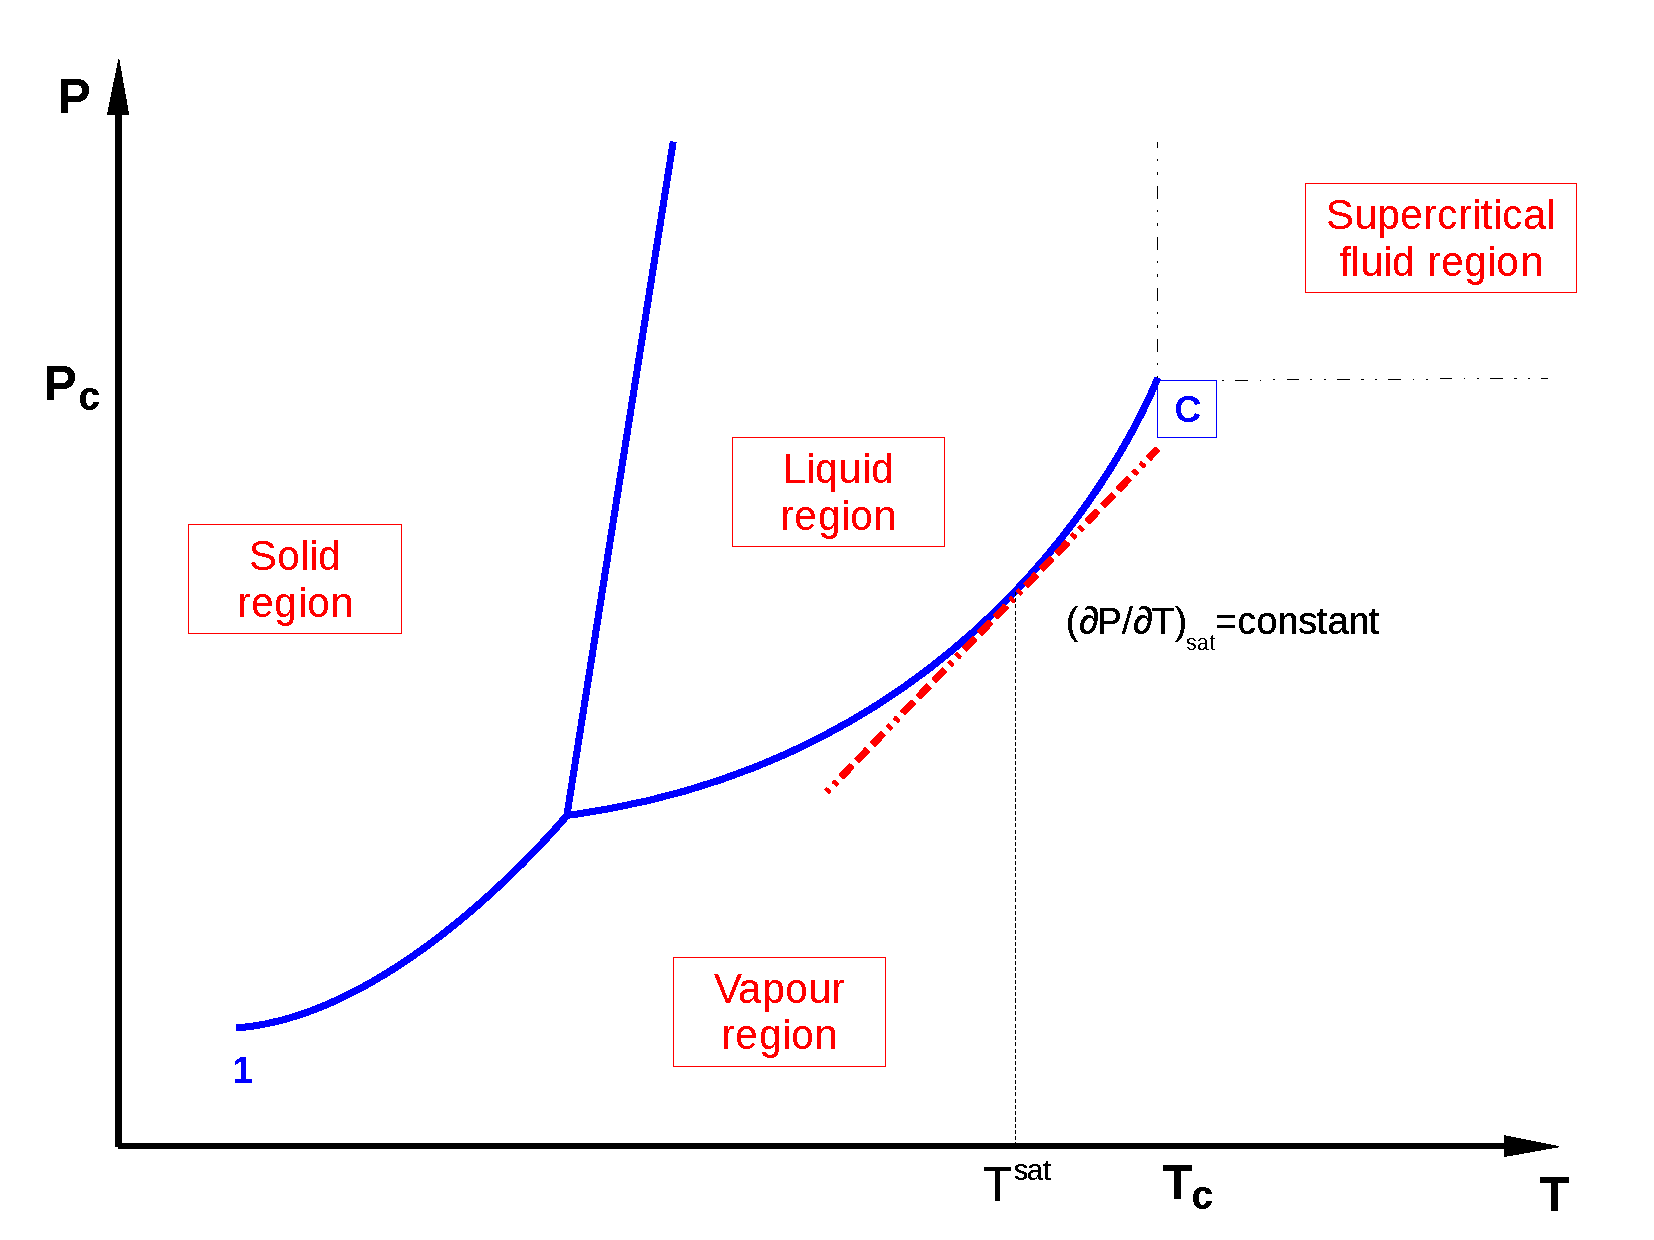
\includegraphics[width=.5\columnwidth,clip]{./../Pics/PT_Diagram2}
               \end{center} 
               \caption{ $PT$ diagrams for a pure substance. Graphical representation of the Clapeyron relation.}\label{Mod03Fig01}
           \end{figure}
      \begin{shaded}
          \begin{equation}
             \frc{d\left(\ln{P^{\text{sat}}}\right)}{dT} = \frc{\Delta H^{\text{fg}}}{RT^{2}} \;\;\Longrightarrow \;\;\; \ln{\left(\frc{P_{2}}{P_{1}}\right)_{\text{sat}}} = \frc{\Delta H^{\text{fg}}}{R}\left(\frc{1}{T_{1}}-\frc{1}{T_{2}}\right)_{\text{sat}}.\label{Mod03_ClausiusClapeyronEqn} 
          \end{equation} 
This expression is known as {\it Clausius-Clapeyron equation} and is a good approximation when describing temperature and pressure dependence at boiling/condensation and at sublimation/gas deposition.
      \end{shaded}
For the dependence of the saturated vapour pressure on $T$, a number of empirical relations have been developed. The simplest expression is,
    \begin{displaymath}
       \ln{P^{\text{sat}}} = A - \frc{B}{T},%\label{Mod03_AntoineSimplest}
    \end{displaymath}
where $A$ and $B$ are constants obtained from experiments. A more `popular' relation is,
    \begin{shaded}
       \begin{equation}
          \ln{P^{\text{sat}}} = A - \frc{B}{T+C},\label{Mod03_Antoine}
       \end{equation}
       this relation is known as {\it Antoine Equation}, where $A$, $B$ and $C$ are constants obtained experimentally.
    \end{shaded}
This two relations, although still widely used by the fluids community are plagued with strong inaccuracy. Due to better accuracy, high-order polynomial relations have become commonly used in flow and process simulators,
    \begin{displaymath}
       \ln{P^{\text{sat}}} = \frc{A\tau + B\tau^{1.5} + C\tau^{3} + D\tau^{6}}{1-\tau}\;\;\;\;\text{ with }\;\;\tau = 1 - T_{r}.
    \end{displaymath}
\end{subequations}


%%% SUBSECTION
   \subsection{Vapour-Liquid Equilibrium Systems}

Several processes of engineering relevance occur with fluids in phase equilibria -- either saturated vapour (\ie vapour saturated with liquid droplets) and saturated liquid (\ie liquid saturated with bubbles of vapour). In most cases, it is important to know the actual quantities of both phases in thermodynamic equilibrium, \ie the amount of vapour and liquid present in a constrained system at prescribed temperature and pressure conditions. Let assume that a closed system contains $n$ moles of a chemical species split into $\mathcal{P}$ phases,
    \begin{displaymath}
      n = \sum\limits_{j=1}^{\mathcal{P}} \mfr[n]{}{j} = \mfr[n]{}{1} + \mfr[n]{}{2} + \cdots + \mfr[n]{}{\mathcal{P}}.
    \end{displaymath}
The mass balance acroos all $\mathcal{P}$ phases can be represented as
    \begin{displaymath}
       nV = \mfr[n]{}{1}\mfr[V]{}{1} + \mfr[n]{}{2}\mfr[V]{}{2} + \cdots + \mfr[n]{}{\mathcal{P}}\mfr[V]{}{\mathcal{P}}  = \sum\limits_{j=1}^{\mathcal{P}}\left(nV\right)^{\left(j\right)},
    \end{displaymath}
where $V$ is the molar volume. Dividing by $n$
    \begin{displaymath}
       V = \frc{\mfr[n]{}{1}}{n}\mfr[V]{}{1} + \frc{\mfr[n]{}{2}}{n}\mfr[V]{}{2} + \cdots + \frc{\mfr[n]{}{\mathcal{P}}}{n}\mfr[V]{}{\mathcal{P}}.
    \end{displaymath}
Defining molar (or mole) fraction, $\mfr[x]{}{j}=\frc{\mfr[n]{}{j}}{n}$, where
    \begin{eqnarray}
         && \sum\limits_{j=1}^{\mathcal{P}}\mfr[x]{}{j} = 1,  \nonumber \\
         && V = \mfr[x]{}{1}\mfr[V]{}{1} + \mfr[x]{}{2}\mfr[V]{}{2} + \cdots + \mfr[x]{}{\mathcal{P}}\mfr[V]{}{\mathcal{P}}.  \nonumber
    \end{eqnarray}
For vapour-liquid systems,
    \begin{eqnarray}
         && \mfr[x]{}{L} + \mfr[x]{}{V} = 1,  \nonumber \\
         && V = \mfr[x]{}{L}\mfr[V]{}{L} + \mfr[x]{}{V}\mfr[V]{}{V}. \nonumber
    \end{eqnarray}
For a generic thermodynamic potential $M$ (= $V$, $U$, $H$, $S$ etc),
    \begin{shaded}
       \begin{subequations}
           \begin{equation}
              M = \left(1-\mfr[x]{}{V}\right)\mfr[M]{}{L} + \mfr[x]{}{V}\mfr[M]{}{V}
           \end{equation}
           \begin{equation}
              M = \mfr[M]{}{L} + \mfr[x]{}{V}\Delta\mfr[M]{}{LV}\label{Mod03_QualityVapour}
           \end{equation}
       \end{subequations}
    \end{shaded}
$\mfr[x]{}{V}$ is called \underline{\it vapour quality}. Thermodynamic potentials of pure substances are graphically represented by $Ph$ (pressure $\times$ specific enthalpy) and $Ts$ (temperature $\times$ specific entropy) diagrams, Fig.~\ref{Mod03Fig02}, where information on $P$, $T$, $s$, $h$, $x$ and $v$ (specific volume) can be readily extracted.
%
           \begin{figure}[h]
              \vbox{
                    \hbox{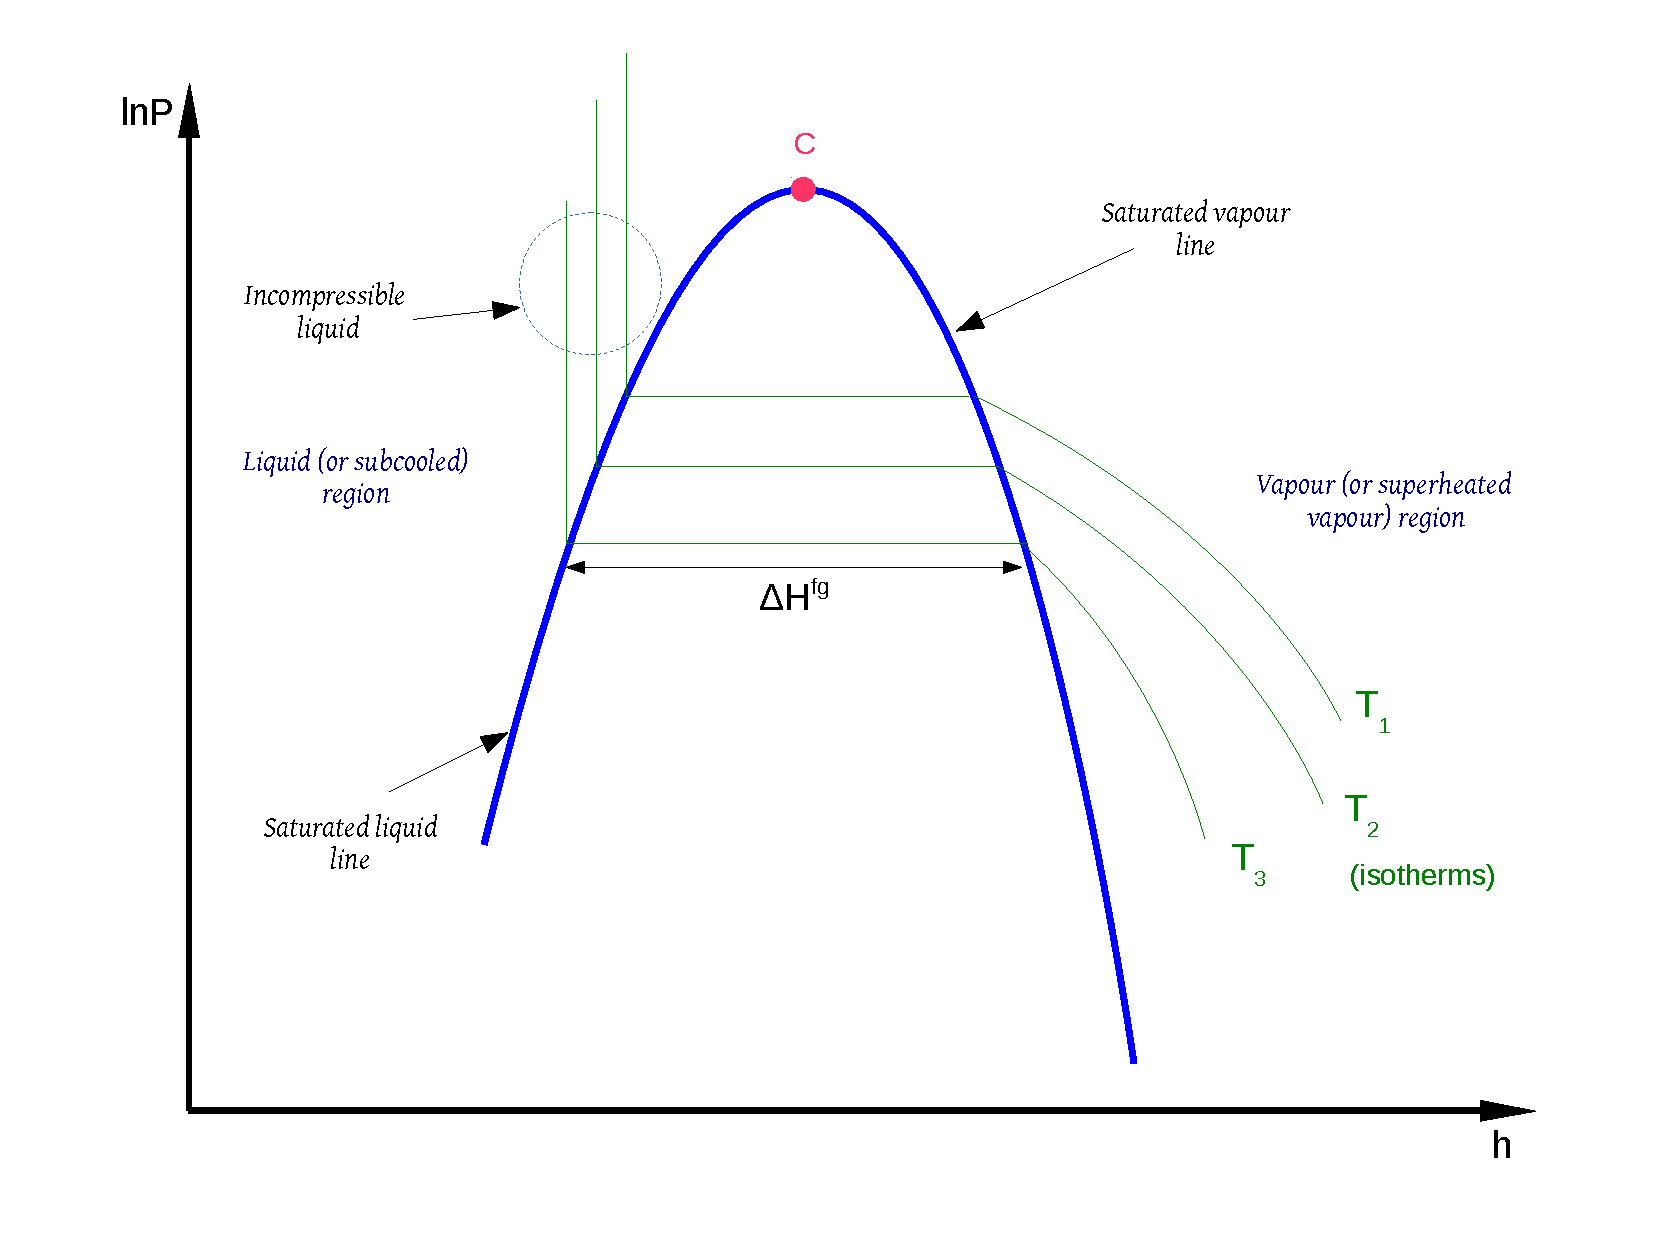
\includegraphics[width=.5\columnwidth,clip]{./Figs/Mod3PHDiagram}
                          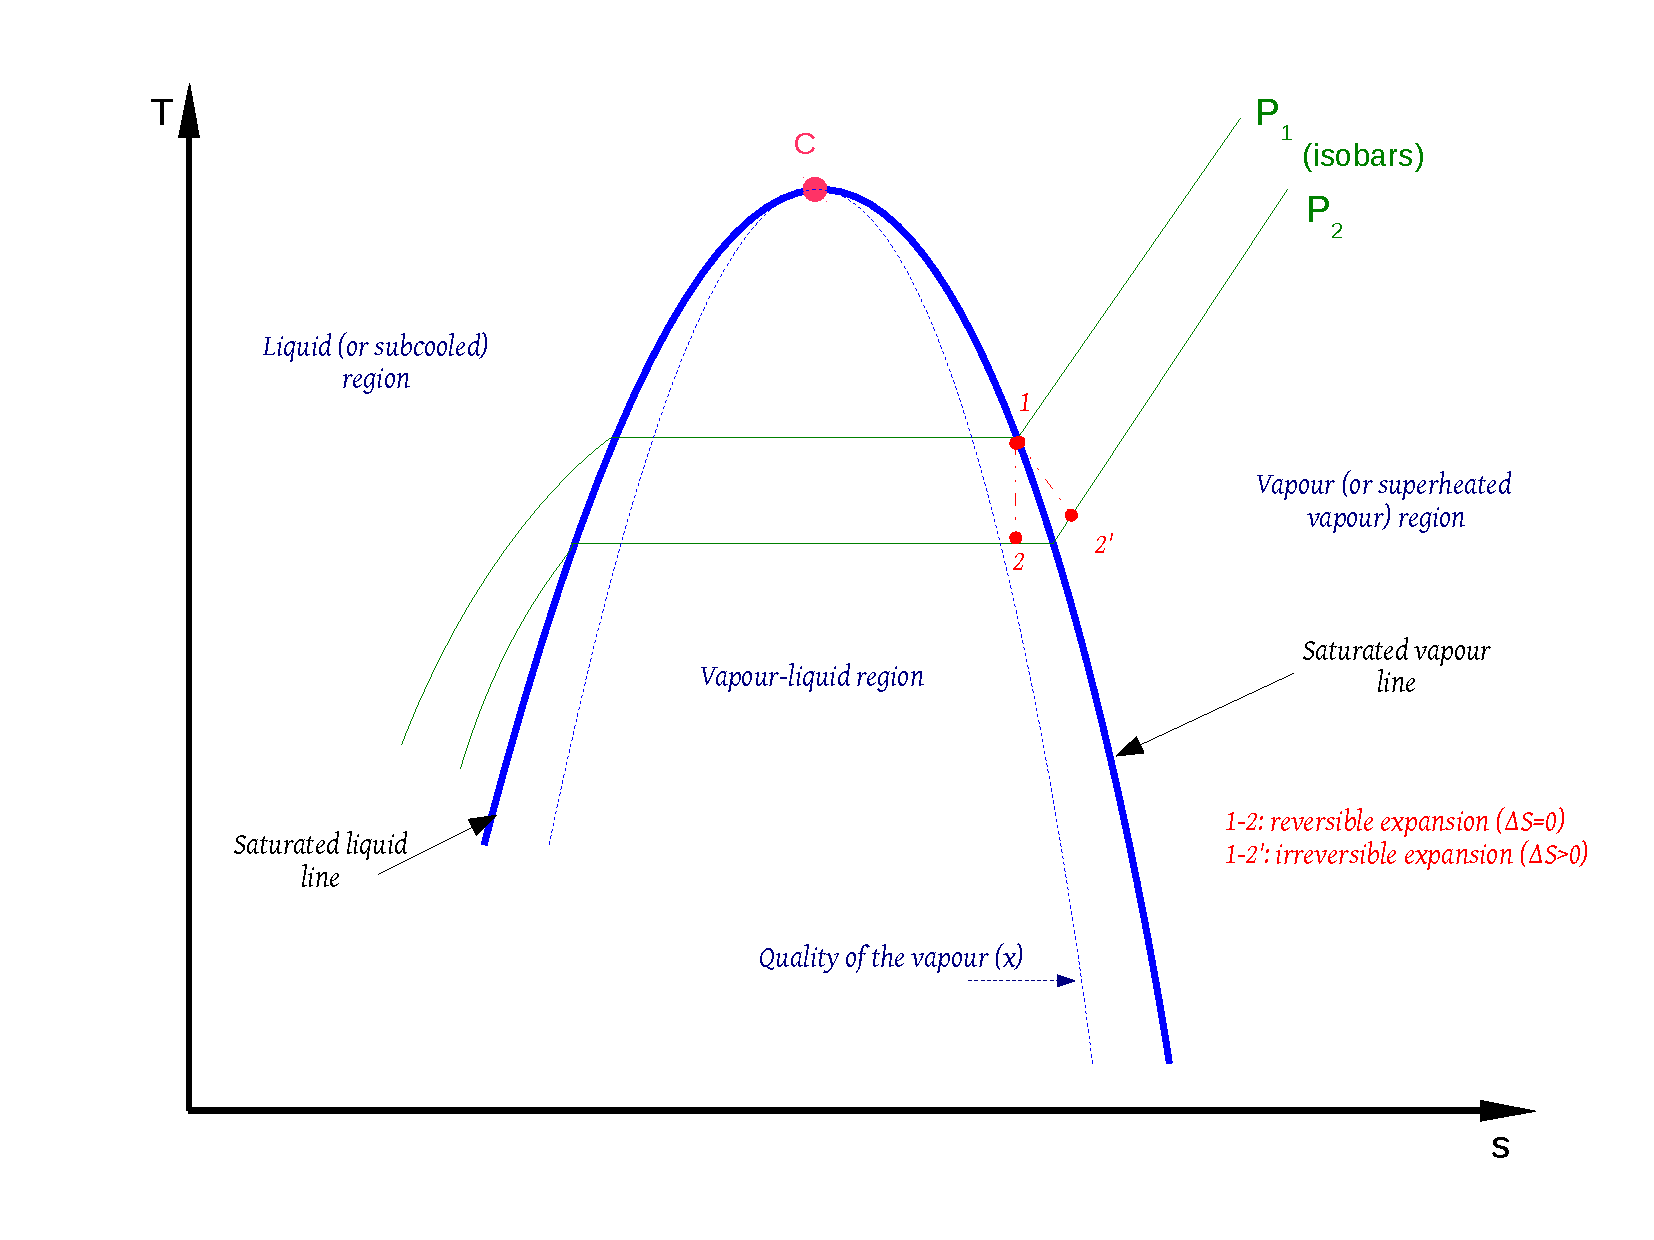
\includegraphics[width=.5\columnwidth,clip]{./Figs/Mod3TSDiagram}}
                    \vspace{-.1cm}
                    \hbox{\hspace{4cm}(a)\hspace{8cm}(b)}}
              \caption{ (a) $Ph$ and (b) $Ts$ diagrams for a pure substance.}\label{Mod03Fig02}
           \end{figure}
%
In the $Ph$ diagram, Fig~\ref{Mod03Fig02}a, isotherms (i.e., lines representing constant temperature) and pressure conditions determine the phase of the fluid. At the left hand-side of the {\it dome} all fluid is at liquid state, whereas at the right hand-side of the {\it dome}, all fluid is at vapour state. The region within the {\it dome} is a two-phase region, where liquid and vapour coexist in thermodynamic equilibrium. As the fluid conditions `move' from the {\it saturated liquid line} to the {\it saturated vapour line} through the {\it isotherm}, the fluid is continuously vaporised `till there is no droplets of liquid fluid. The total amount of heat given to the system -- $\Delta H^{\text{fg}}$, is the latent heat of vaporisation. In a similar way, the $Ts$ diagram, Fig~\ref{Mod03Fig02}b, shows similar features over different {\it isobars}. In addition, the {\it quality} of the vapour can also be graphically represented. In a reversible expansion from $P_{1}$ to $P_{2}$ $\left(P_{1}>P_{2}\right)$, entropy change is null, $\Delta s=0$, and is represented by a vertical line, however during irreversible expansion, $\Delta s >0$, represented by an inclined line.  

 $Ph$ and $Ts$ diagrams for common substances are no longer used by industry but it helps to qualitatively understand phase (and associated thermodynamic potentials) behaviour of pure substances. Quantitative information can be obtained from either saturated and superheated (Fig.~\ref{Mod03Fig03}) fluid tables or dedicated software, \eg
\begin{itemize}
   \item \href{http://www.weatherford.com/doc/wft183650}{PVTflex$^{TM}$};
   \item \href{http://www.kbcat.com/infochem-software/flow-assurance-software-multiflash/pvt-simulation}{Multiflash$^{TM}$};
   \item \href{https://www.honeywellprocess.com/en-US/explore/products/advanced-applications/unisim/Pages/default.aspx}{UniSim – Software for Process Design and Simulation};
   \item \href{http://webbook.nist.gov/chemistry/fluid/}{NIST Website}
   \item etc.
\end{itemize}
In general, table of {\it saturated fluid properties}, Fig.~\ref{Mod03Fig03}a, contains information of the fluid within the {\it dome}, whereas the table of {\it superheated fluid properties} refer to the region outside (rhs) the {\it dome}. 
%
   \begin{figure}[h]
      \vbox{
         \hbox{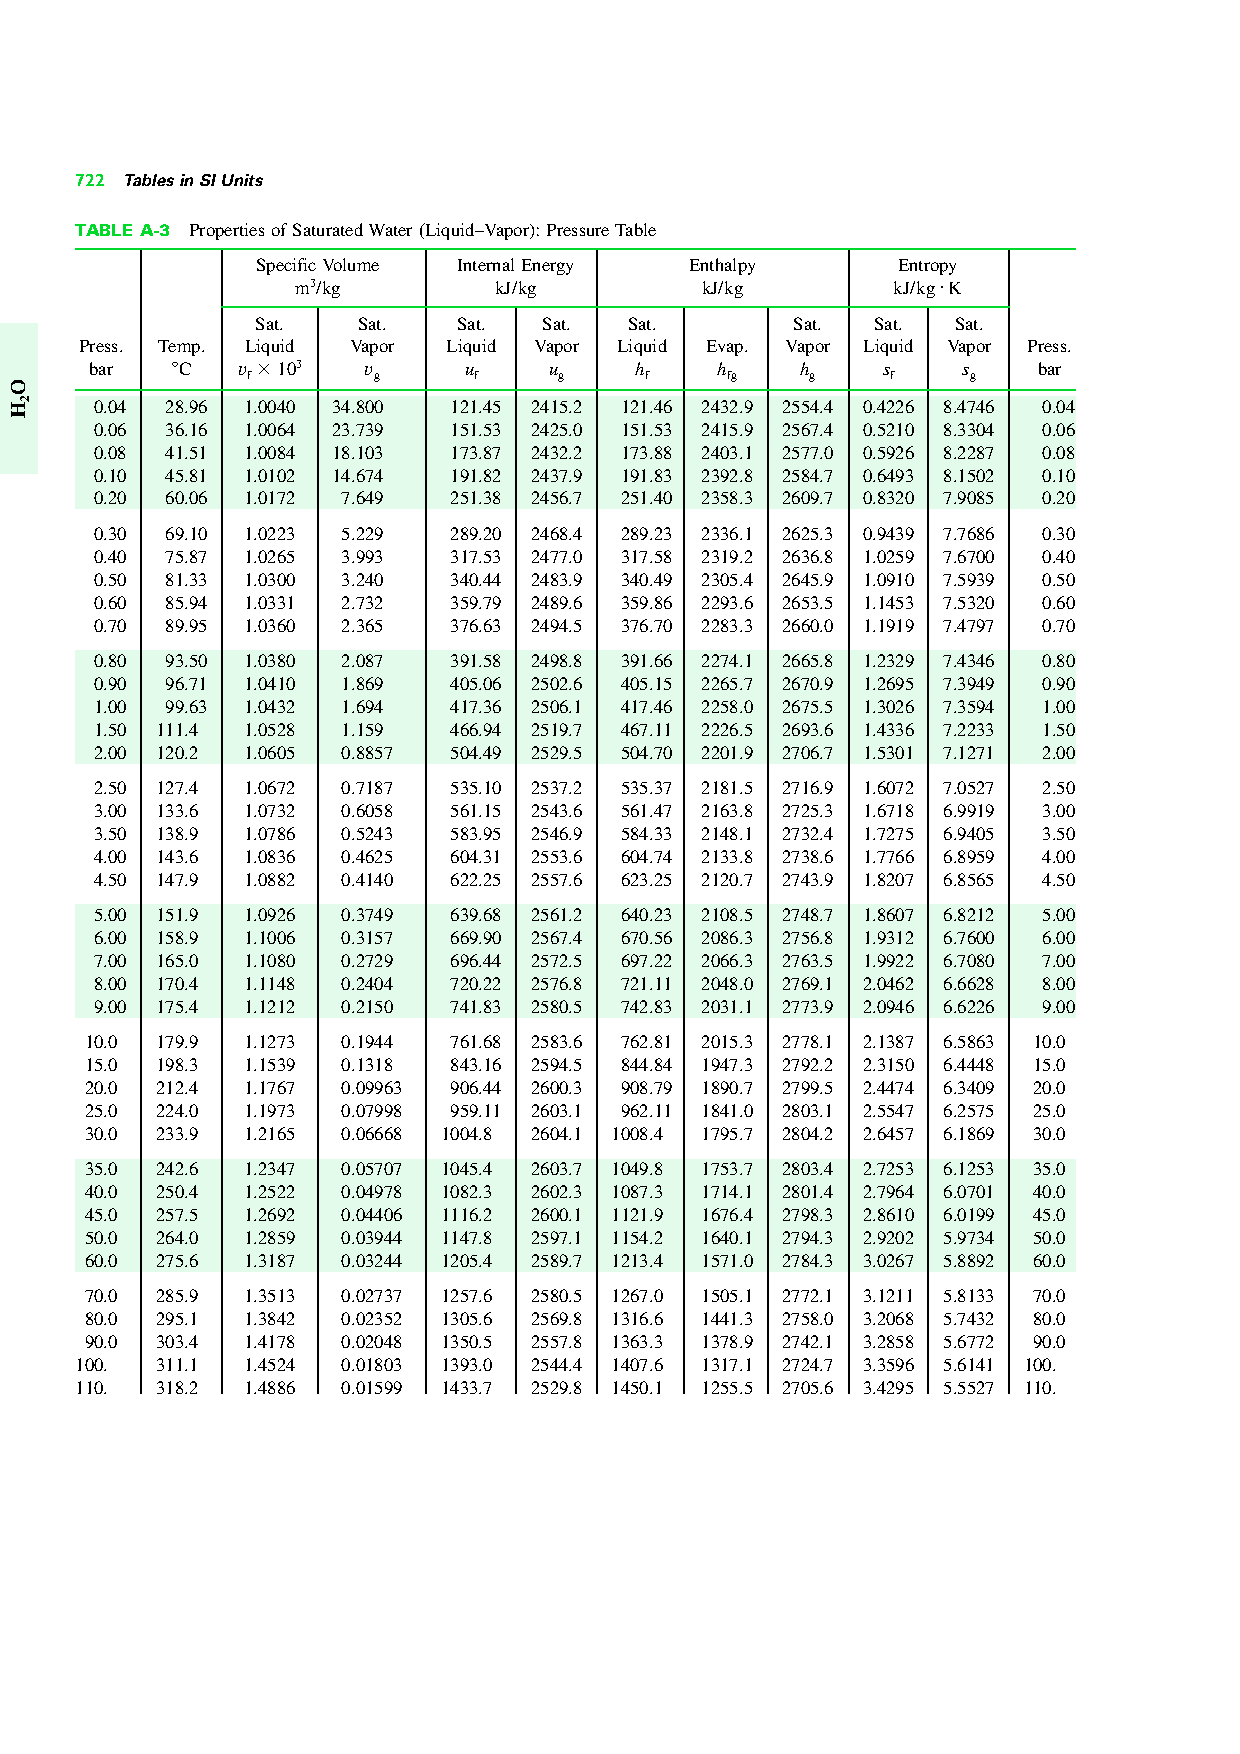
\includegraphics[width=.5\columnwidth,clip]{./Figs/WaterSatTable}
               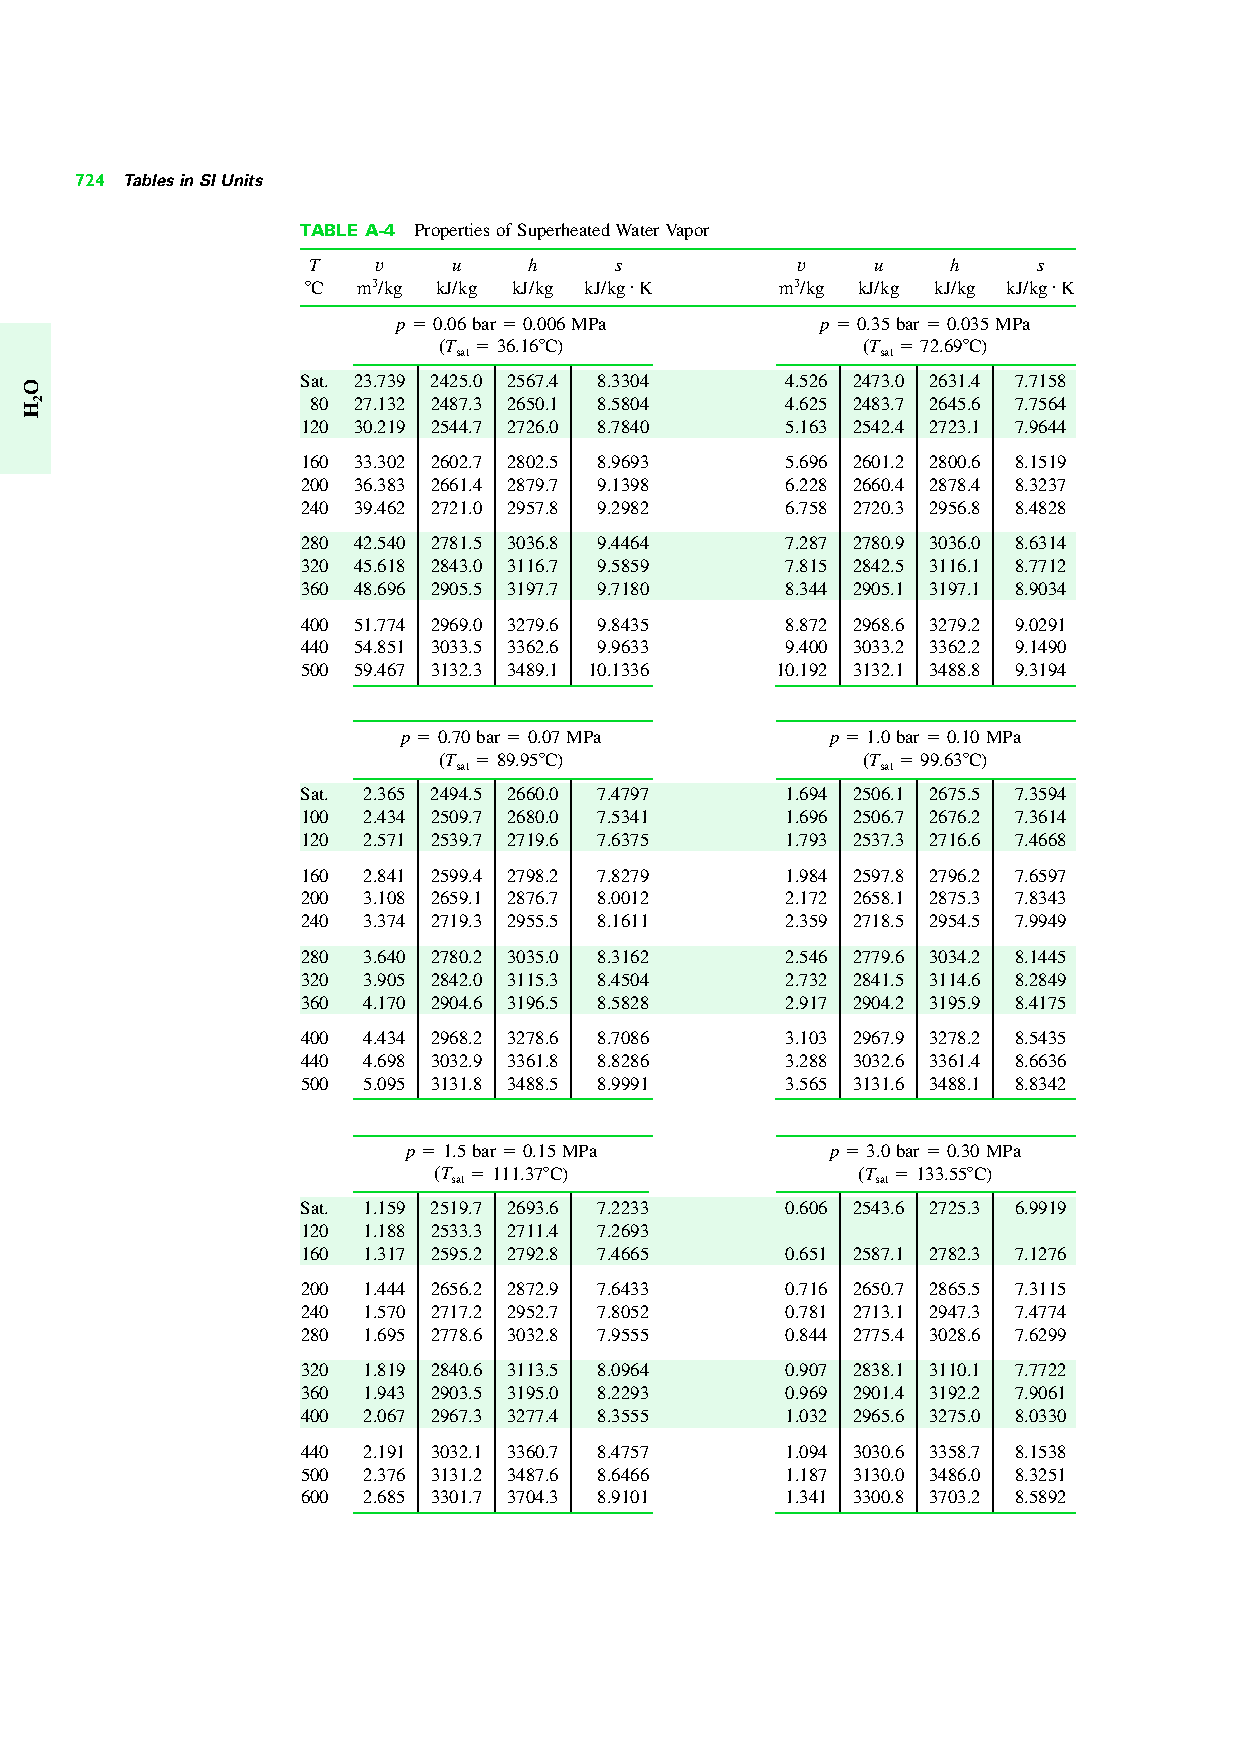
\includegraphics[width=.5\columnwidth,clip]{./Figs/Water_SuperheatedTable}}
         \vspace{-1.5cm}
         \hbox{\hspace{4cm}(a)\hspace{7cm}(b)}
      }
      \caption{ Table of properties of (a) saturated water-steam and (b) superheated vapour (Extracted from Moran $\&$ Saphiro, see Appendix B).}\label{Mod03Fig03}  
   \end{figure}
%
    

%%% SUBSECTION
   \subsection{Industrial Applications: Power System}
Regardless the energy source (fossil fuel, nuclear or geothermal), power plants are good applications for VLE systems as fluids are continuously vaporised and condensed by addition and extraction of heat and volume expansion. {\it Rankine thermal cycles} are system configurations for generating power and consist of four processes (Fig.~\ref{Mod03Fig04}) with associated energy balances:
     \begin{itemize}
      \item \textcolor{red}{Process 1-2}: reversible adiabatic (i.e., \blue{isentropic}) expansion in the turbine (or steam engine),
            \begin{displaymath}
               \left(h_{2} + \dot{W}_{T}\right)-h_{1} = 0 \Rightarrow \dot{W}_{T} = h_{1}-h_{2}
            \end{displaymath}
      \item \textcolor{red}{Process 2-3}: constant-pressure heat transfer (to the environment) in the condenser,
            \begin{displaymath}
               \left(h_{3} + \dot{Q}_{C}\right)-h_{2} = 0 \Rightarrow \dot{Q}_{C} = h_{2}-h_{3}
            \end{displaymath}
      \item \textcolor{red}{Process 3-4}: reversible adiabatic (i.e., \blue{isentropic}) pumping process in the feed pump,
            \begin{displaymath}
               h_{4} - \left(h_{3} + \dot{W}_{P}\right) = 0 \Rightarrow \dot{W}_{P} = h_{4}-h_{3}
            \end{displaymath}
      \item \textcolor{red}{Process 4-1}: constant-pressure heat transfer (to the fluid) in the boiler,
            \begin{displaymath}
               h_{1} - \left(h_{4} + \dot{Q}_{B}\right) = 0 \Rightarrow \dot{Q}_{B} = h_{1}-h_{4}
            \end{displaymath} 
     \end{itemize}
     The efficiency $\left(\eta\right)$ of the Rankine cycle is given by
           \begin{displaymath}
               \eta_{\text{Rankine}} = \frc{\sum W_{i}}{Q_{B}} = \frc{\left|W_{\text{net}}\right|}{Q_{B}} = \frc{\left|\left(h_{1}-h_{2}\right)+\left(h_{4}-h_{3}\right)\right|}{h_{1}-h_{4}}.
           \end{displaymath}
     Due to engineering constraints, fluids entering and leaving the pump \underline{must be} at liquid phase, thus $h_{4}=h_{f4}$ and $h_{3}=h_{f3}$, \ie the fluid has the enthalpy of the liquid phase (from the saturated fluid table) at the prescribed temperature and pressure conditions. {\it Pumps} are able to induce the transport of liquid fluids that are often assumed incompressible, therefore
          \begin{displaymath}
                Tds = dh - v dP
          \end{displaymath}
as the compression occurs isentropically, \ie $ds=0$,
          \begin{displaymath}
                dh = v dP \Rightarrow h_{f4} = h_{f3} + v_{3}\left(P_{4}-P_{3}\right).
          \end{displaymath}
However, as $\left(h_{f4}-h_{f3}\right) <<<<< \left(h_{1}-h_{2}\right)$, the efficiency can be considered as
           \begin{displaymath}
               \eta_{\text{Rankine}} = \frc{\left|\left(h_{1}-h_{2}\right)\right|}{h_{1}-h_{f4}}.
           \end{displaymath}     
%
   \begin{figure}[h]
      \begin{center}
         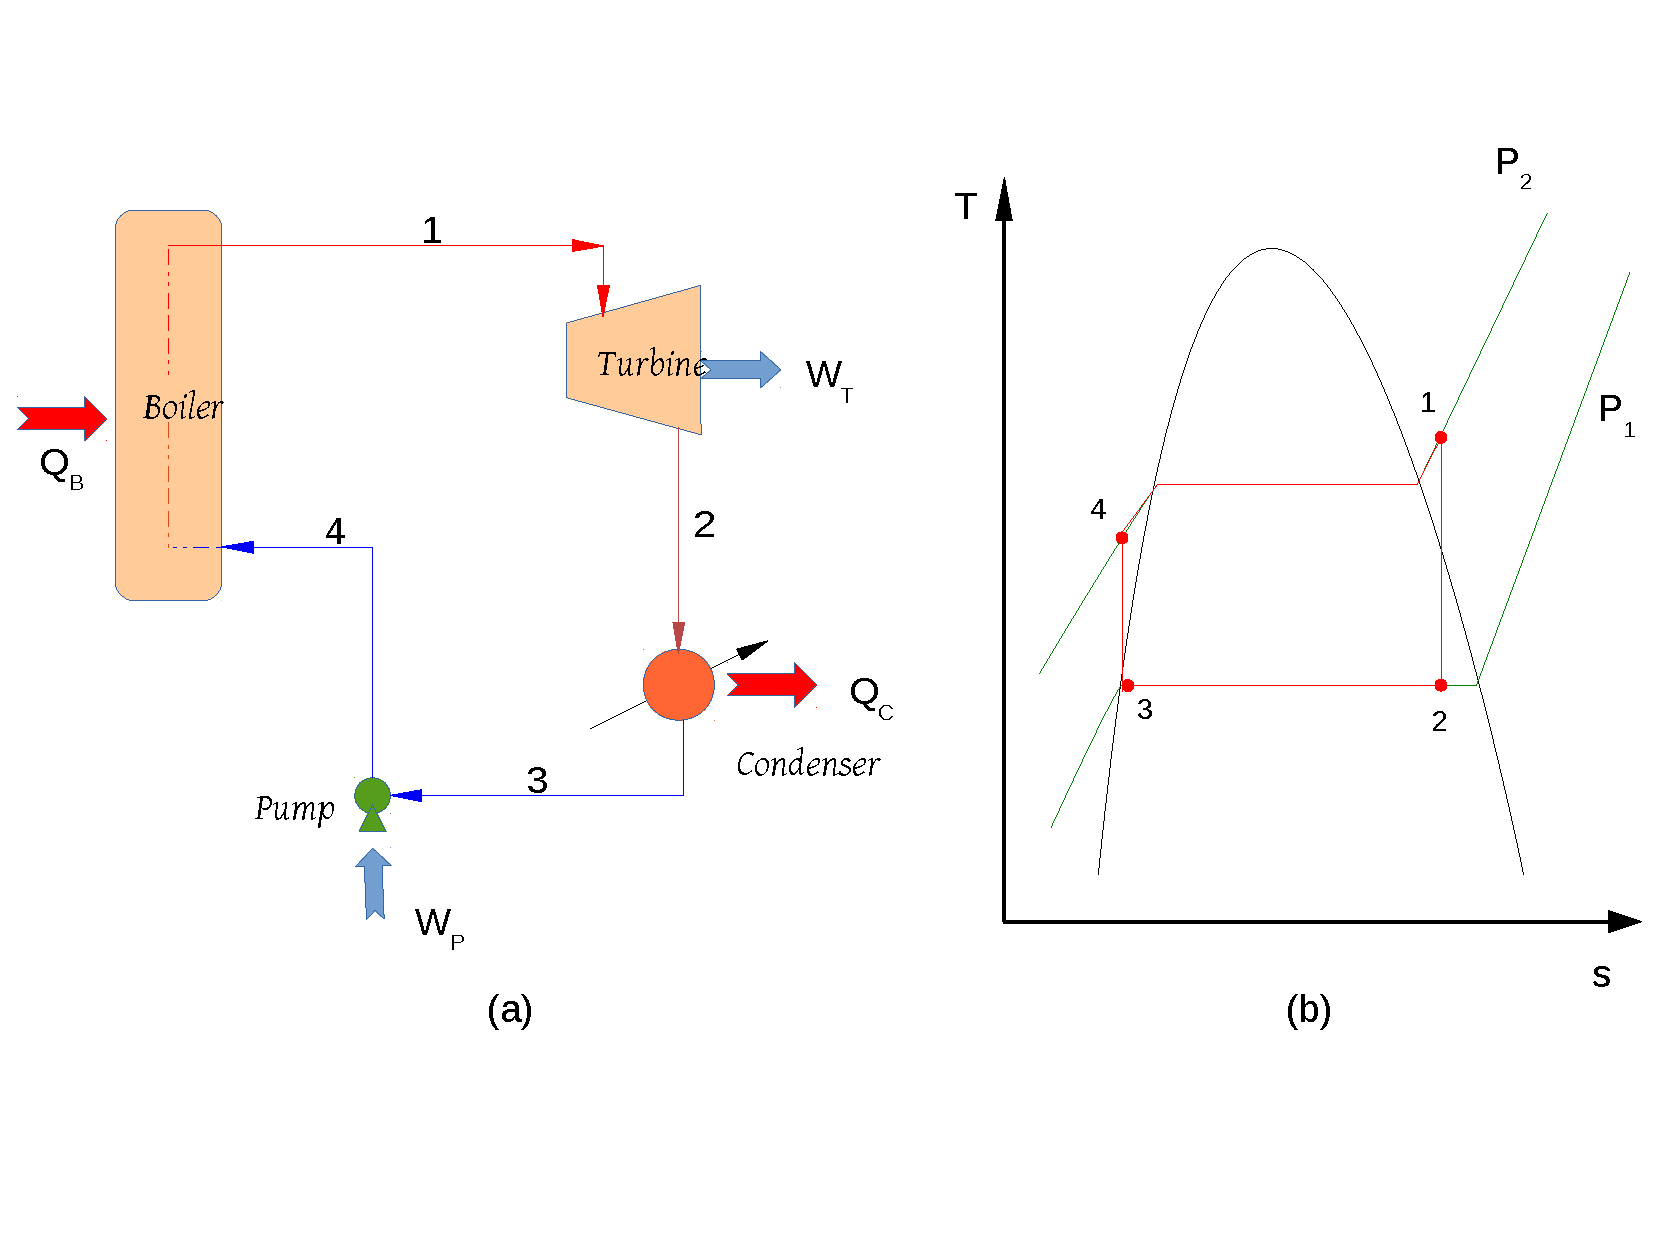
\includegraphics[width=\columnwidth,clip]{./Figs/Mod3PowerSystemDiagram}
      \end{center}
      \caption{ (a) Diagram of Rankine thermal cycle for power generation and associated $Ts$ diagram.}\label{Mod03Fig04}
   \end{figure}


\clearpage

%%% SECTION
\section{Examples}
       \begin{enumerate}

%%%
%%% EXAMPLE 
%%%
\item\label{Mod03Ex03} The Antoine equation constants for toluene are $A=14.01415$, $B=3106.46$ K and $C=-53.15$ K (for pressure given in kPa). At 1.01325$\times$10$^{5}$ Pa, calculate the boiling temperature and the enthalpy of vaporisation at this temperature.

% SOLUTION
    \noindent{\bf Solution:} Boiling temperature can be calculated from the Antoine equation,
       \begin{displaymath}
          \ln{P^{\text{sat}}} = A - \frc{B}{T+C} \;\;\;\Rightarrow \;\;\; T = \frc{B}{A-\ln{P^{\text{sat}}}} - C = \red{383.77 K}
       \end{displaymath}
The enthalpy of vaporisation, $\Delta H^{\text{fg}}$, can be obtained from the Clausius-Clapeyron equation,
         \begin{eqnarray}
            \frc{d}{dT} \left(\ln{P^{\text{sat}}}\right) &=& \frc{\Delta H^{\text{fg}}}{RT^{2}} \nonumber \\
             \frc{B}{\left(T+C\right)^{2}} &=&  \frc{\Delta H^{\text{fg}}}{RT^{2}} \;\;\Longrightarrow \Delta H^{\text{fg}} = 34.7984 \text{kJ.mol}^{-1}. \nonumber
         \end{eqnarray}
 
\clearpage

%%%
%%% EXAMPLE 
%%%  
\item\label{Mod03Ex04} Derive an expression for enthalpy change of a gas during an isothermal process assuming using the following EOS: $P\left(V-b\right)=RT$

% SOLUTION
    \noindent{\bf Solution:} We have seen that enthalpy change is given by Eqn.~\ref{Mod03_DerivedEnthalpyRelation1},
    \begin{displaymath}
       dH = C_{p}dT + \left[V - T\Partial[V]{T}{P}\right]dP.
    \end{displaymath}
    We can rearrange the given EOS and obtain $\Partial[V]{T}{P}$,
    \begin{eqnarray}
       && P\left(V-b\right)=RT \;\;\;\rightarrow\;\;\; V = \frc{RT}{P} + b \;\;\;\rightarrow\;\;\; \Partial[V]{T}{P} = \frc{R}{P}\;\;\text{ thus, } \nonumber \\
       && dH = C_{p}dT + \left(V - \frc{RT}{P}\right)dP = \blue{C_{p}dT + bdP}. \nonumber 
    \end{eqnarray}
    
\clearpage
    
\clearpage
 
%%%
%%% EXAMPLE 
%%%  
\item\label{Mod03Ex06} Steam (dry and saturated) is supplied by the boiler at 15 bar and the condenser inlet pressure is 0.4 bar. Calculate the Rankine efficiency of the cycle. Neglect the pump work, assume the enthalpy of fluid leaving the pump is 317.58 kJ.kg$^{-1}$

% SOLUTION  
    \noindent{\bf Solution:} At 15 bar, dry and saturated $\left(\ie x_{1}=1\right)$ steam has the following properties (from saturated table)\footnote{Using the same numbering as in Fig.~\ref{Mod03Fig04}.},
          \begin{eqnarray}
             T_{1} &=& T_{\text{sat}} = 198.3^{\circ}\text{C},\nonumber \\
             h_{1} &=& h_{\text{g}} = 2792.2\; \text{kJ.kg}^{-1} \nonumber \\
             s_{1} &=& s_{\text{g}} = 6.4448\; \text{kJ.(kg.K)}^{-1} \nonumber
          \end{eqnarray} 
    In the condenser, $P_{2}=0.4$ bar,
          \begin{eqnarray}
              T_{2} &=& T_{\text{sat}} = 75.87^{\circ}\text{C}, \nonumber \\
              h_{\text{g}2} &=& 2636.8\;\text{kJ.kg}^{-1},\;\;\; h_{\text{f}2} = 317.58\;\text{kJ.kg}^{-1},  \nonumber \\
              s_{\text{g}2} &=& 7.6700 \;\text{kJ.(kg.K)}^{-1},\;\;\; s_{\text{f}2} = 1.0259\;\text{kJ.(kg.K)}^{-1}. \nonumber  
          \end{eqnarray}
$h_{2}$ and $s_{2}$ depend on the knowledge of how vaporised the water is, in other words, we need to determine the quality of the steam, $x_{1}$ through Eqn.~\ref{Mod03_QualityVapour},
      \begin{eqnarray}
          h_{2} &=& h_{\text{f}2} + x_{2}\left(h_{\text{g}2} - h_{\text{f}2}\right), \nonumber \\
          s_{2} &=& s_{\text{f}2} + x_{2}\left(s_{\text{g}2} - s_{\text{f}2}\right). \nonumber
      \end{eqnarray}
As we know that water is expanded isentropically in the turbine, \ie $s_{1}=s_{2}$,
      \begin{displaymath}
         s_{2} = s_{\text{f}2} + x_{2}\left(s_{\text{g}2} - s_{\text{f}2}\right) = s_{1} = 6.4448 \;\;\;\Rightarrow \;\;\; x_{2} = 0.8156 \;\;(81.56\% \text{ of vapour}
      \end{displaymath}
Thus replacing in 
      \begin{displaymath}
          h_{2} = h_{\text{f}2} + x_{2}\left(h_{\text{g}2} - h_{\text{f}2}\right) = 2209.14\text{ kJ.kg}^{-1}.
      \end{displaymath}
The Rankine efficiency is given by
      \begin{displaymath}
           \eta_{\text{Rankine}} = \frc{\text{Adiabatic or Isentropic Heat Drop}}{\text{Heat Supplied}} = \frc{\left|h_{1}-h_{2}\right|}{h_{1}-h_{\text{f}4}} = 0.2356\;\;\;\rightarrow \;\;\; 23.56\%
      \end{displaymath}
    


\end{enumerate}


